\documentclass[a4paper,12pt]{article}
\usepackage{acn-scientific}
\usepackage{acn-questions}

\title{Fraunhofer Alphabet}
\author{\textsc{A.C. Norman}
\\ \texttt{a.norman@olcc.lancs.sch.uk}}
\date{}

%\showanswerstrue
\showanswersfalse

\begin{document}

\thispagestyle{empty}

\maketitle

\noindent Based on \emph{Fraunhofer Alphabet} Alan Winter 1980 \emph{Phys. Educ.} \textbf{15} 291; diffraction patterns simulated in python using accompanying code from Adams, C.S.\ \& Hughes, I.G.\ \emph{Optics f2f: From Fourier to Fresnel}, OUP (2018)

\vfill

\begin{itemize}
\item The diffraction patterns of capital letters are shown below.
\item The patterns are in alphabetical order. 
\item There are 22 (out of 26 possible) patterns; four letters are missing.
\end{itemize}

\vfill

Your task is to identify:
\begin{enumerate}
    \item Which are the four missing letters?
    \item Sketch what you expect each of the missing diffraction patterns to look like.
\end{enumerate}

\thispagestyle{empty}

\vfill

\begin{center}
\begin{tikzpicture}[x={(0.866cm,-0.3cm)}, y={(0.866cm,0.5cm)}, z={(0cm,1cm)}, scale=2]
% Opaque mask
\draw[fill=gray!150] (-0.5,2,-0.5)-- (0.5,2,-0.5)-- (0.5,2,0.5)-- (-0.5,2,0.5)node[above]{letter-shaped aperture}--(-0.5,2,-0.5);
% Question-mark aperture
\begin{scope}
    \pgftransformcm
        {1.732}{-0.6}
        {0}{2}
        {\pgfpoint{3.22cm/2.6}{1.88cm/2.6}}

    \pgftext[left,bottom]{
       \Large \sffamily \textcolor{white}{\textbf{?}}
     }
\end{scope}
%slit:
%\draw[fill] (-0.5,2,-0.5)-- (-0.05,2,-0.5)-- (-0.05,2,0.5)-- (-0.5,2,0.5)node[above]{letter-shaped aperture}--(-0.5,2,-0.5);
%\draw[fill] (0.05,2,-0.5)-- (0.5,2,-0.5)-- (0.5,2,0.5)-- (0.05,2,0.5)--(0.05,2,-0.5);
%beam:
\draw[ultra thick,gray] (0,0,0)node[left,black]{laser} -- (0,2,0);
% Diffraction pattern filling screen
\begin{scope}
    \pgftransformcm
        {1.732}{-0.6}
        {0}{2}
        {\pgfpoint{3.22cm}{1.88cm}}

    \pgftext[left,bottom]{
        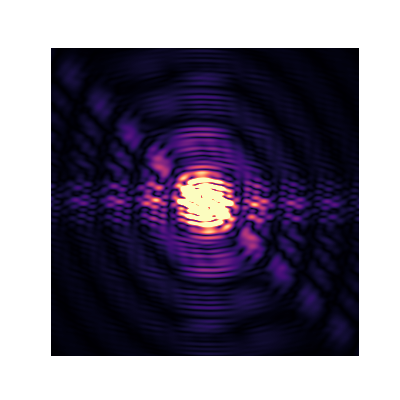
\includegraphics[width=1cm,height=1cm]{img/?.png}
    }
\end{scope}
%screen:
\draw[thick] (-1,5,-1)-- (1,5,-1)-- (1,5,1)-- (-1,5,1)node[above]{pattern on screen}--(-1,5,-1);
\end{tikzpicture}
\end{center}

\vfill

% ANSWER: E, I, N, U

\newpage

\begin{center}
    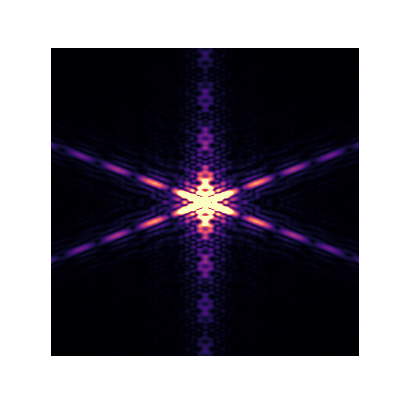
\includegraphics[width=0.26\textwidth]{img/A.png}   \hspace{-1.4em}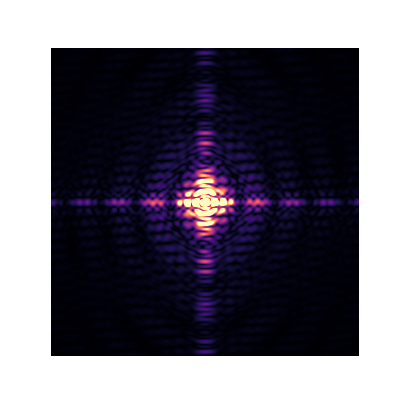
\includegraphics[width=0.26\textwidth]{img/B.png}
    \hspace{-1.4em}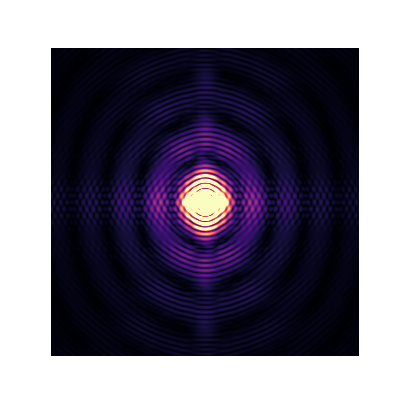
\includegraphics[width=0.26\textwidth]{img/C.png}
    \hspace{-1.4em}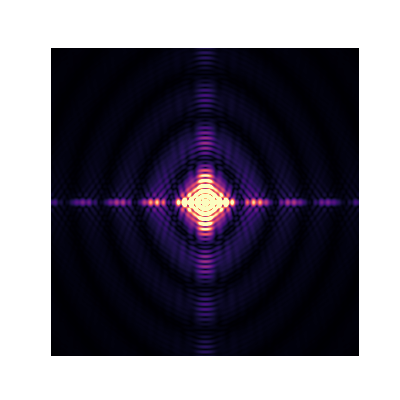
\includegraphics[width=0.26\textwidth]{img/D.png}

      \vspace{-1.4em}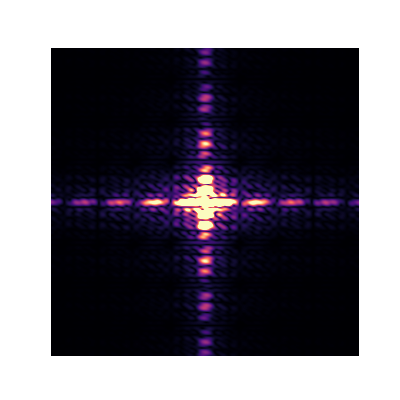
\includegraphics[width=0.26\textwidth]{img/F.png}   \hspace{-1.4em}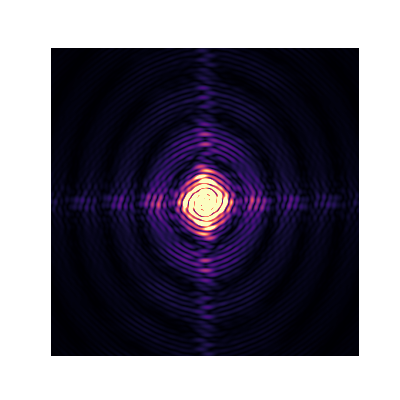
\includegraphics[width=0.26\textwidth]{img/G.png}
    \hspace{-1.4em}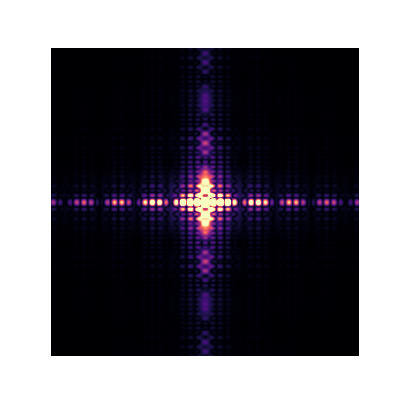
\includegraphics[width=0.26\textwidth]{img/H.png}
    \hspace{-1.4em}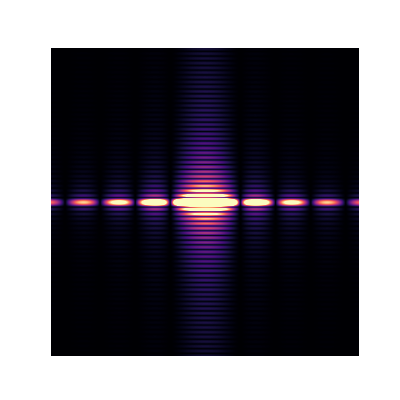
\includegraphics[width=0.26\textwidth]{img/J.png}

      \vspace{-1.4em}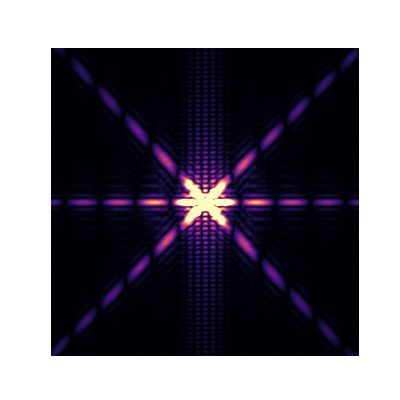
\includegraphics[width=0.26\textwidth]{img/K.png}   \hspace{-1.4em}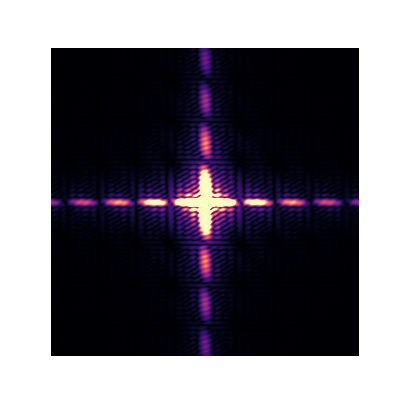
\includegraphics[width=0.26\textwidth]{img/L.png}
    \hspace{-1.4em}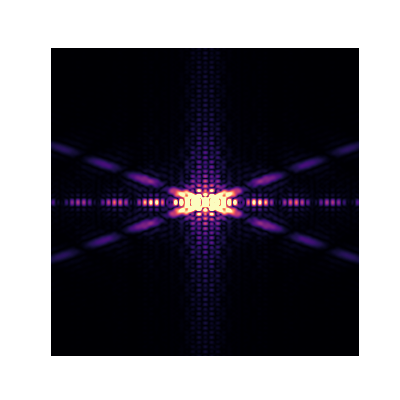
\includegraphics[width=0.26\textwidth]{img/M.png}
    \hspace{-1.4em}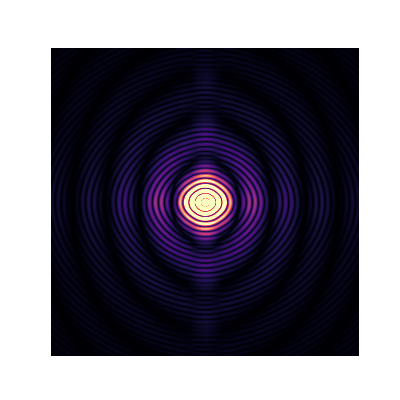
\includegraphics[width=0.26\textwidth]{img/O.png}

      \vspace{-1.4em}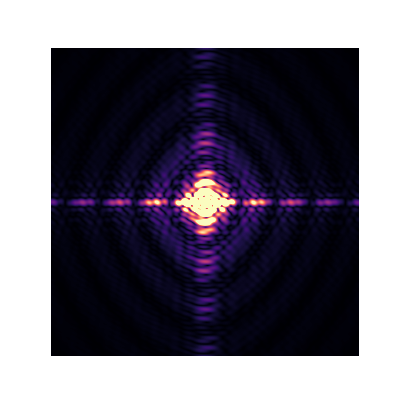
\includegraphics[width=0.26\textwidth]{img/P.png}   \hspace{-1.4em}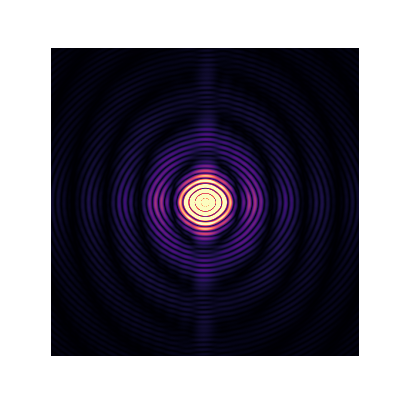
\includegraphics[width=0.26\textwidth]{img/Q.png}
    \hspace{-1.4em}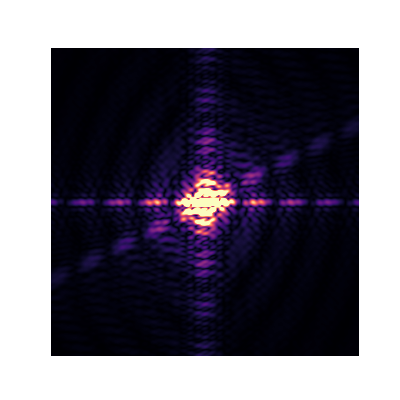
\includegraphics[width=0.26\textwidth]{img/R.png}
    \hspace{-1.4em}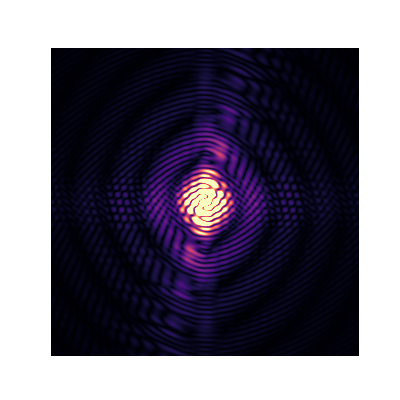
\includegraphics[width=0.26\textwidth]{img/S.png}

      \vspace{-1.4em}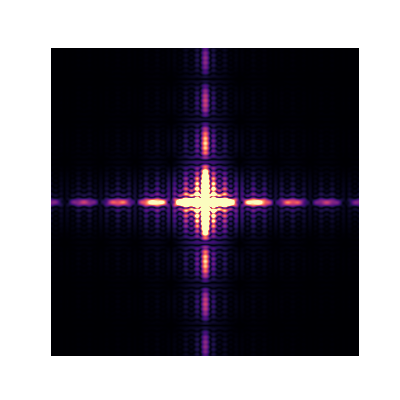
\includegraphics[width=0.26\textwidth]{img/T.png}   \hspace{-1.4em}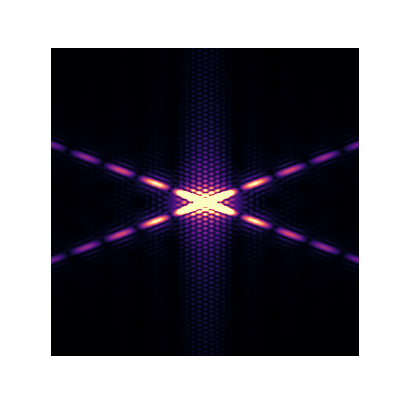
\includegraphics[width=0.26\textwidth]{img/V.png}
    \hspace{-1.4em}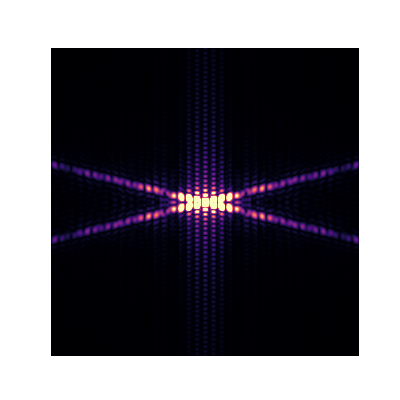
\includegraphics[width=0.26\textwidth]{img/W.png}
    \hspace{-1.4em}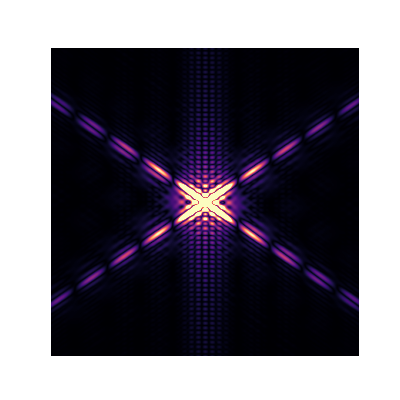
\includegraphics[width=0.26\textwidth]{img/X.png}

       \vspace{-1.4em}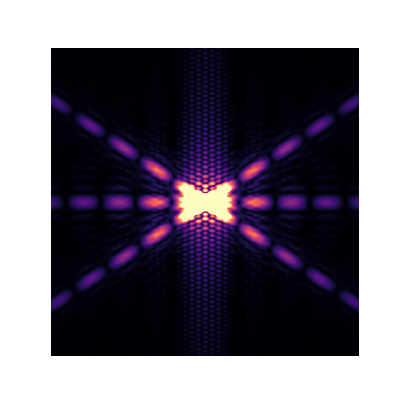
\includegraphics[width=0.26\textwidth]{img/Y.png}   \hspace{-1.4em}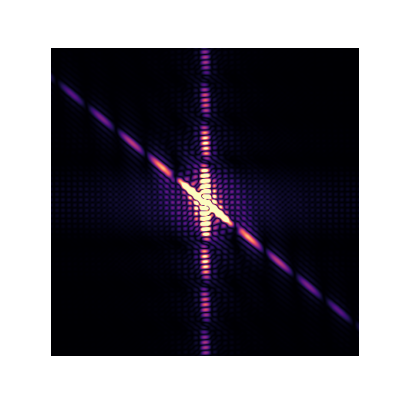
\includegraphics[width=0.26\textwidth]{img/Z.png}
    \hspace{-1.4em}\phantom{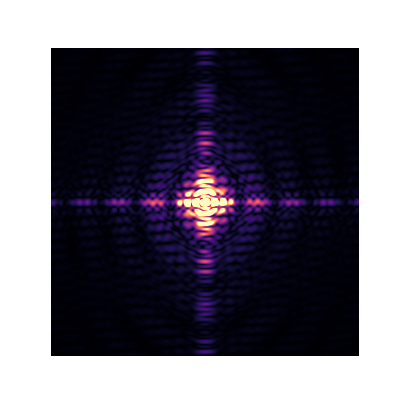
\includegraphics[width=0.26\textwidth]{img/B.png}}
    \hspace{-1.4em}\phantom{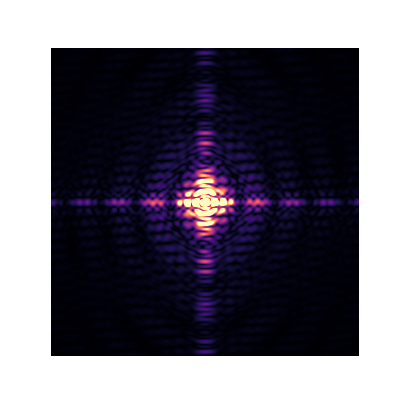
\includegraphics[width=0.26\textwidth]{img/B.png}}

\enlargethispage{1cm}

\end{center}

%\vfill
%\ccbyncsa
\end{document}